\documentclass[10pt]{beamer}

% Beamer style
%\usetheme[secheader]{Madrid}
% \usetheme{CambridgeUS}
\useoutertheme{infolines}
\usecolortheme[rgb={0.65,0.15,0.25}]{structure}
% \usefonttheme[onlymath]{serif}
\beamertemplatenavigationsymbolsempty
%\AtBeginSubsection

% Packages
%\usepackage[french]{babel}
\usepackage[latin1]{inputenc}
\usepackage{color}
\usepackage{xspace}
%\usepackage{dsfont, stmaryrd}
\usepackage{amsmath, amsfonts, amssymb}
\usepackage{url}
\usepackage{/home/robin/LATEX/Biblio/astats}
%\usepackage[all]{xy}
\usepackage{graphicx}
\usepackage{tikz}
\newcommand{\nodesize}{2em}
\newcommand{\edgeunit}{1*\nodesize}
\tikzstyle{node}=[point, inner sep=0]
\tikzstyle{edge}=[-, line width=.5pt]

% Not numbering backup slides
\newcommand{\backupbegin}{
   \newcounter{finalframe}
   \setcounter{finalframe}{\value{framenumber}}
}
\newcommand{\backupend}{
   \setcounter{framenumber}{\value{finalframe}}
}


% Commands
\definecolor{darkred}{rgb}{0.65,0.15,0.25}
\newcommand{\emphase}[1]{\textcolor{darkred}{#1}}
% \newcommand{\emphase}[1]{{#1}}
\newcommand{\paragraph}[1]{\textcolor{darkred}{#1}}
\newcommand{\refer}[1]{{\footnotesize{\textcolor{gray}{[{\cite{#1}}]}}}}
\newcommand{\Refer}[1]{{\footnotesize{\textcolor{gray}{[{#1}]}}}}
\renewcommand{\newblock}{}

% Symbols
\newcommand{\Abf}{{\bf A}}
\newcommand{\Beta}{\text{B}}
\newcommand{\Bcal}{\mathcal{B}}
\newcommand{\BIC}{\text{BIC}}
\newcommand{\Ccal}{\mathcal{C}}
\newcommand{\dd}{\text{~d}}
\newcommand{\dbf}{{\bf d}}
\newcommand{\Dcal}{\mathcal{D}}
\newcommand{\Esp}{\mathbb{E}}
\newcommand{\Espt}{\widetilde{\Esp}}
\newcommand{\Ebf}{{\bf E}}
\newcommand{\Ecal}{\mathcal{E}}
\newcommand{\Gcal}{\mathcal{G}}
\newcommand{\Gam}{\mathcal{G}\text{am}}
\newcommand{\Hcal}{\mathcal{H}}
\newcommand{\Ibb}{\mathbb{I}}
\newcommand{\Ibf}{{\bf I}}
\newcommand{\ICL}{\text{ICL}}
\newcommand{\Cov}{\mathbb{C}\text{ov}}
\newcommand{\Corr}{\mathbb{C}\text{orr}}
\newcommand{\Var}{\mathbb{V}}
\newcommand{\Vsf}{\mathsf{V}}
\newcommand{\pen}{\text{pen}}
\newcommand{\pt}{\widetilde{p}}
\newcommand{\Fcal}{\mathcal{F}}
\newcommand{\Hbf}{{\bf H}}
\newcommand{\Jcal}{\mathcal{J}}
\newcommand{\Kbf}{{\bf K}}
\newcommand{\Lcal}{\mathcal{L}}
\newcommand{\Mcal}{\mathcal{M}}
\newcommand{\mbf}{{\bf m}}
\newcommand{\mum}{\mu(\mbf)}
\newcommand{\Ncal}{\mathcal{N}}
\newcommand{\Nbf}{{\bf N}}
\newcommand{\Nm}{N(\mbf)}
\newcommand{\Ocal}{\mathcal{O}}
\newcommand{\Obf}{{\bf 0}}
\newcommand{\Omegas}{\underset{s}{\Omega}}
\newcommand{\Pbf}{{\bf P}}
\newcommand{\Pt}{\widetilde{P}}
\newcommand{\Pcal}{\mathcal{P}}
\newcommand{\Qcal}{\mathcal{Q}}
\newcommand{\Rbb}{\mathbb{R}}
\newcommand{\Rcal}{\mathcal{R}}
\newcommand{\Scal}{\mathcal{S}}
\newcommand{\Ucal}{\mathcal{U}}
\newcommand{\Vcal}{\mathcal{V}}
\newcommand{\BP}{\text{BP}}
\newcommand{\EM}{\text{EM}}
\newcommand{\VEM}{\text{VEM}}
\newcommand{\VBEM}{\text{VBEM}}
\newcommand{\cst}{\text{cst}}
\newcommand{\obs}{\text{obs}}
\newcommand{\ra}{\emphase{\mathversion{bold}{$\rightarrow$}~}}
%\newcommand{\transp}{\text{{\tiny $\top$}}}
\newcommand{\transp}{\text{{\tiny \mathversion{bold}{$\top$}}}}
\newcommand{\logit}{\text{logit}\xspace}

% Directory
\newcommand{\figmixt}{/home/robin/ENSEIGN/COURS/MELANGE}
\newcommand{\figbma}{/home/robin/RECHERCHE/RUPTURES/MELANGE/Exemples/Grippe}
\newcommand{\fignet}{../FIGURES}
\newcommand{\figeco}{/home/robin/RECHERCHE/ECOLOGIE/EXPOSES/FIGURES}
%\newcommand{\figmotif}{/home/robin/RECHERCHE/RESEAUX/Motifs/FIGURES}


%====================================================================
%====================================================================

%====================================================================
%====================================================================
\begin{document}
%====================================================================
%====================================================================

%====================================================================
\title[$W$-graphs and their inference]{$W$-graphs and their inference \\ ~\\
  \normalsize{(with emphasize en variational Bayes)}}

\author[S. Robin]{S. Robin + P. Latouche, S. Ouadah}

\institute[INRA/AgroParisTech]{INRA / AgroParisTech \\ ~\\
  \vspace{-.1\textwidth}
  \begin{tabular}{ccccc}
%     
\includegraphics[height=.3\textheight]{\fignet/LogoINRA-Couleur} & 
%     \hspace{.02\textheight} &
%     
\includegraphics[height=.08\textheight]{\fignet/logagroptechsolo} & 
%     \hspace{.02\textheight} &
%     
\includegraphics[height=.09\textheight]{\fignet/logo-ssb}
    
\includegraphics[height=.2\textheight]{\fignet/LogoINRA-Couleur} & 
    \hspace{.02\textheight} &
    
\includegraphics[height=.067\textheight]{\fignet/logagroptechsolo} & 
    \hspace{.02\textheight} &
    
\includegraphics[height=.06\textheight]{\fignet/logo-ssb}
    \\ 
  \end{tabular} \\
  \bigskip
  }

\date[COSTNET, Sept.'16]{COSTNET, Ribno, September 2016}

%====================================================================
%====================================================================
\maketitle
%====================================================================

%====================================================================
%====================================================================
\section{Exchangeable graphs}
\frame{\frametitle{Outline} \tableofcontents[currentsection]}
%====================================================================
\frame{ \frametitle{Some notations}

  \paragraph{Graph $\Gcal = (\Vcal, \Ecal)$:}
  $\Vcal =$ vertices $:= \{1, \dots n\}$, $\Ecal =$ edges $\subset \Vcal \times \Vcal$
  
  \bigskip \bigskip 
  \paragraph{Adjacency matrix $Y = [Y_{ij}]$:}
  $$
  Y: n \times n, \qquad Y_{ij} = \Ibb\{(i, j) \in \Ecal\}
  $$
 
  \bigskip
  \paragraph{Random graph:} defined by the joint distribution of all edges
  $$
  p(Y) = p\left( [Y_{ij}] \right)
  $$

  \bigskip 
  \paragraph{Undirected graph:}
%   $\{(i, j) \in \Ecal\} \Leftrightarrow \{(j, i) \in \Ecal\}$
%   that is 
  $Y_{ij} = Y_{ji}$
  
  }

%====================================================================
\frame{ \frametitle{Exchangeability}

  \paragraph{Classical exchangeability:} % $(Y_1, \dots Y_n)$ exchangeable iff
  for any permutation $\sigma$
  $$
  P([Y_i=y_i]) = P([Y_i=y_{\sigma(i)}]).
  $$
  
  
  \bigskip \bigskip
  \paragraph{Joint exchangeability} for two dimensional arrays \refer{DiJ08}: % $[Y_{ij}]$ jointly exchangeable iff 
  $$
  P([Y_{ij}]=[y_{ij}]) = P([Y_{ij}]=[y_{\emphase{\sigma}(i)\emphase{\sigma}(j)}])
  $$
  for any permutation $\sigma$ (applied to both $i$ and $j$).

  \bigskip \pause
  $$
  \left(
  \begin{tabular}{p{.9\textwidth}}
  \paragraph{Separate exchangeability:}  
  $P([Y_{ij}]=[y_{ij}]) = P([Y_{ij}]=[y_{\emphase{\sigma}(i)\emphase{\tau}(j)}])$ \\
  for any permutations $\sigma$ and $\tau$ \ra directed graphs.   
  \end{tabular}
  \right)
  $$
%   \paragraph{Separate exchangeability:} 
%   $$
%   P(\forall i, j: Y_{ij}=y_{ij}) = P(\forall i, j: Y_{ij}=y_{\emphase{\sigma}(i)\emphase{\tau}(j)})
%   $$
%   for any permutations $\sigma$ and $\tau$ \ra directed graphs.
  }

%====================================================================
\frame{ \frametitle{Aldous-Hoover theorem}

  \paragraph{Theorem:} $Y = [Y_{ij}]$ is exchangeable iff there exists $F: [0, 1]^3 \mapsto \{0, 1\}$,
  $$
  [Y_{ij}] \overset{d}{=} [F(U_i, U_j, U_{ij})]
  $$
  where $(U_i)_i$ and $(U_{ij})_{i, j}$ are iid $\Ucal[0, 1]$.
  
  \bigskip \bigskip \pause
  \paragraph{Properties:}
  \begin{itemize}
   \item The $Y_{ij}$'s are not independent (because of the $U_i$'s and $U_j$'s) \\~
   \item \pause The $Y_{ij}$'s are conditionally independent given the $U_i$'s:
   $$
   [Y_{ij}] | (U_i = u_i)_i \overset{d}{=} [F(u_i, u_j, U_{ij})]
   $$
  \end{itemize}

}

%====================================================================
\frame{ \frametitle{Some exchangeable random graphs}

  \paragraph{State-space models:} 
  \begin{eqnarray*}
   \{Z_i\}_i \text{ iid} & \sim & \pi \\
   \{Y_{ij}\}_{ij} \text{ indep. } | \; \{Z_i\}_i & \sim & \Bcal[\gamma(Z_i, Z_j)]
  \end{eqnarray*}
 
  \bigskip \pause
  \begin{itemize}
  \item Latent space \refer{HRH02}*: $Z_i \in \Rbb^d, \quad \gamma(Z_i, Z_j) = f(\|Z_i-Z_j\|)$
  \item Model-based clustering \refer{HRT07}: $\pi =$ Gaussian mixture, 
  \item Stochastic bloc-model (SBM) \refer{HoL79,NoS01}: $\pi = \Mcal, \quad \gamma = [\gamma_{k\ell}]$
  \item Continuous version of SBM \refer{DPV10}*: $Z_i \in \Scal^d$
  \item $W$-graph \refer{LoS06,DiJ08}: $\pi = \Ucal_{[0, 1]}$
  \end{itemize}
%   See \Refer{Matias \& R. (2014)}\nocite{MaR14} for a review:
  See \refer{MaR14} for a statistical review + \refer{BJR07} for theoretical properties.
  
  \bigskip
  \footnotesize{(*): $Z_i$ not explicitly random}
}

% %====================================================================
% \frame{ \frametitle{SBM and $W$-graph}
% 
%   \paragraph{SBM:} $\pi = (\pi_1, \dots \pi_K)$ group proportions, $[\gamma_{k\ell}] =$ connexion probabilities
%   \begin{eqnarray*}
%    \{Z_i\}_i \text{ iid} & \sim & \Mcal(1; \pi) \\
%    \{Y_{ij}\}_{ij} \text{ indep. } | \; \{Z_i\}_i & \sim & \Bcal[\gamma_{Z_i, Z_j}] 
%   \end{eqnarray*}
% 
%   \bigskip \bigskip \pause 
%   \paragraph{$W$-graph:} denote $w: [0, 1]^2 \mapsto [0, 1]$ the \emphase{graphon} function:
%   \begin{eqnarray*}
%    \{U_i\}_i \text{ iid} & \sim & \Ucal_{[0, 1]} \\
%    \{Y_{ij}\}_{ij} \text{ indep. } | \; \{U_i\}_i & \sim & \Bcal[w(U_i, U_j)] \\
%    ~ \\
%    \Rightarrow F(U_i, U_j, U_{ij}) & = & \Ibb\{U_{ij} < w(U_i, U_j)\}
%   \end{eqnarray*}
% 
% }

%====================================================================
%====================================================================
\section{$W$-graph \& graphon function}
%====================================================================
\frame{ \frametitle{$W$-graph}

  \begin{tabular}{cc}
    \hspace{-.02\textwidth}
    \begin{tabular}{p{.5\textwidth}}
    \begin{itemize}
     \item \emphase{Graphon} function: 	 
	 $$w: [0, 1]^2 \mapsto [0, 1]$$
	 \item \pause $\{U_i\}_i \text{ iid} \sim \Ucal_{[0, 1]}$ \\~
	 \item \pause $\{Y_{ij}\}_{ij} \text{ indep. } | \; \{U_i\}_i$:
	 $$Y_{ij} | U_i, U_j \sim \Bcal[w(U_i, U_j)]$$
    \end{itemize}
    \end{tabular}
    & 
    \hspace{-.1\textwidth}
    \begin{tabular}{p{.5\textwidth}}
	 Graphon function $w(u, u')$ \\
      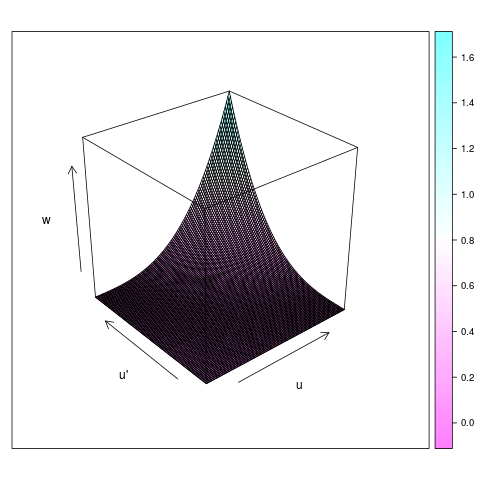
\includegraphics[width=.5\textwidth]{../FIGURES/FigCLADAG-W-graphon2} \\
    \end{tabular}
  \end{tabular}
  
  \pause \bigskip 
  \paragraph{Aldous-Hoover representation:}
  $
  F(U_i, U_j, U_{ij}) = \Ibb\{U_{ij} < w(U_i, U_j)\}
  $

}

%====================================================================
\frame{ \frametitle{Some ideal graphons}

  \begin{tabular}{p{.12\textwidth}p{.3\textwidth}p{.12\textwidth}p{.3\textwidth}}
    \begin{tabular}{r} 'Scale free' \end{tabular} & 
    \begin{tabular}{c} 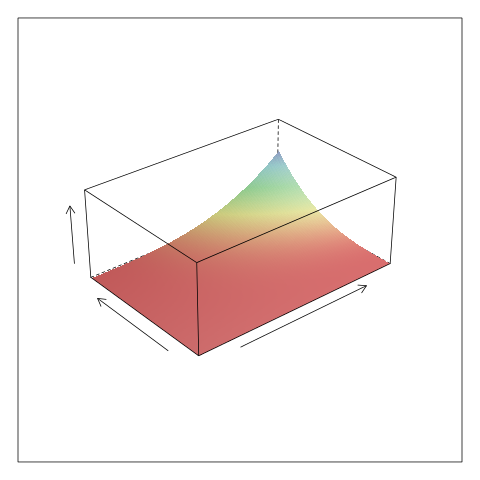
\includegraphics[width=.3\textwidth]{../FIGURES/EDD-ScaleFreeTrueGraphon} \end{tabular} & 
    \begin{tabular}{r} Community \end{tabular} &
    \begin{tabular}{c} 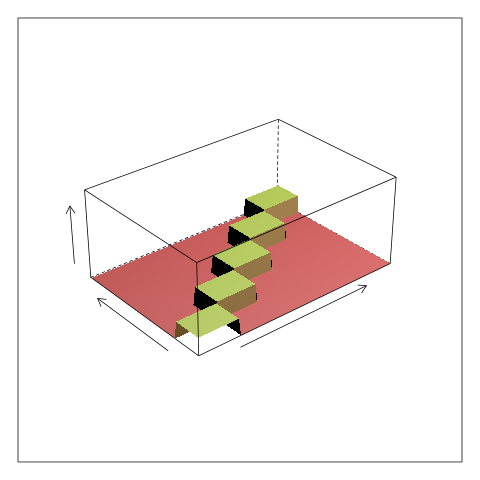
\includegraphics[width=.3\textwidth]{../FIGURES/CommunityTrueGraphon} \end{tabular} \\
    \begin{tabular}{r} SBM \end{tabular} & 
    \begin{tabular}{c} 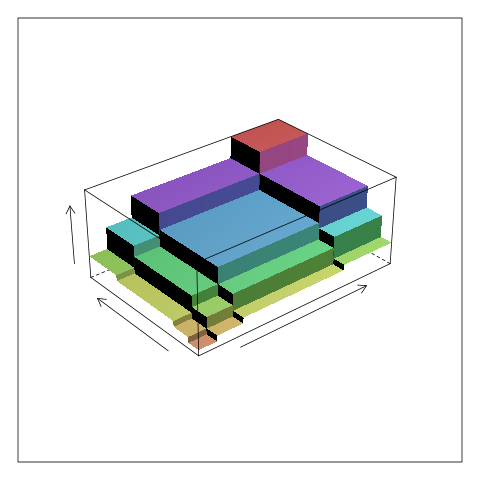
\includegraphics[width=.3\textwidth]{../FIGURES/SBMGraphon} \end{tabular} &
    \begin{tabular}{r} Small world  \end{tabular} &
    \begin{tabular}{c} 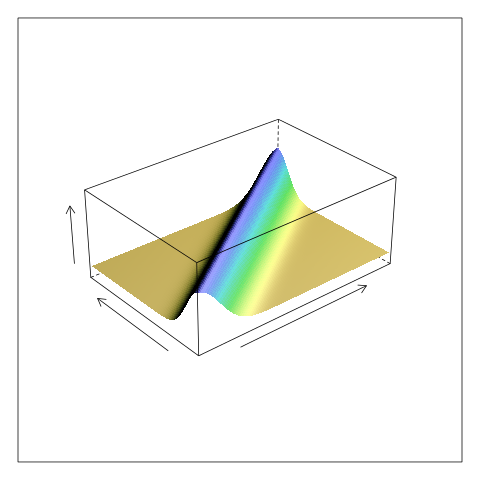
\includegraphics[width=.3\textwidth]{../FIGURES/SmallWorldTrueGraphon}  \end{tabular}
  \end{tabular}
  
  }

%====================================================================
\frame{ \frametitle{$W$-graph as limit for dense graphs}

  \paragraph{Asymptotic framework:} (a crude rephrasing of \refer{LoS06,DiJ08})
  \begin{itemize}
   \item $(\Gcal_n) =$ sequence of exchangeable graphs with increasing size (say $n$)
   \item $t(F, G) =$ number of occurrences of subgraph $F$ (with $k$ nodes) in $G$ normalized by $n_{[k]}$.
  \end{itemize}
  
  \pause \bigskip \bigskip
  \paragraph{Convergence:} If for any finite set of fixed subgraphs $(F_1, \dots F_m)$, $(t(F_1, \Gcal_n), \dots t(F_m ,\Gcal_n))$ converge in distribution, \\
  then 
  \begin{itemize}
  \item there exist a $W$-graph $\Gcal$ such that $(\Gcal_n) \overset{d}{\longrightarrow} \Gcal$;
  \item for any fixed $F$, $\Esp t(F, \Gcal_n) \longrightarrow f(F)$ where
  $$
  f(F) = \int_{[0, 1]^{k}} \prod_{(i, j) \in \Ecal(F)} w(u_i, u_j) \dd u_1 \dots \dd u_{k}
  $$
  \end{itemize}
}

%====================================================================
\frame{ \frametitle{Some comments}

  \paragraph{Questions}
  \begin{itemize}
   \item How strong is the condition 
   $$
   (t(F_1, \Gcal_n), \dots t(F_m ,\Gcal_n)) \text{ converge in distribution?}
   $$
   \item Does it hold for most popular state-space models?
   \item Does it hold for other popular state graph models (e.g. ERGM \refer{FrS86})?
  \end{itemize}
  
  \pause \bigskip \bigskip 
  \paragraph{Comments:} If so
  \begin{itemize}
   \item One should be able to derive the graphon of any of these models.
   \item Only pairwise interactions (asymptotically) matter.
   \item More complex patterns (e.g. triangles in ERGM) are (asymptotically) useless.
  \end{itemize}

}

%====================================================================
\frame{ \frametitle{Identifiability}

  \paragraph{Obvious identifiability problem:} consider $\phi: [0, 1] \mapsto [0, 1]$ measure preserving, then the two graphons 
  $$
  w(u, v) \qquad \text{and} \qquad w'(u, v) = w(\phi(u), \phi(v))
  $$ 
  give raise to the same random graph \refer{DiJ08,YHA14}.
  
  \pause \bigskip \bigskip
  \paragraph{Degree function:} Denoting $D_i = \sum_{j \neq i} Y_{ij}$, $\Esp (D_i | U_i = u) = (n-1) g(u)$,
  $$
  g(u) = \int_{[0, 1]} w(u, v) \dd v.
  $$

  \pause \bigskip 
  \paragraph{Identifiability condition \refer{BiC09,YHA14,ChA14}:} 
  $$
  g(u) \text{ strictly increasing.}
  $$ 

}

%====================================================================
%====================================================================
\section{Statistical inference}
\frame{\frametitle{Outline} \tableofcontents[currentsection]}
%====================================================================
\frame{ \frametitle{Infering $w$}
  
  \paragraph{Main issues}
  \begin{itemize}
   \item $W$-graph is a state-space for graph = incomplete data model \\
    \ra Specificity of graph models: $p([U_i] | Y)$ intractable\footnote{due to graph moralization}. \\ ~
   \item $W$-graph is a graph model \\
    \ra No prior ordering of the nodes is given in general.
  \end{itemize}

  \pause \bigskip \bigskip
  \paragraph{Specificity of $W$-graph}
  \begin{itemize}
   \item Recent interest in the statistical community (since 2014) \\
    \ra but explosion since then. \\~ 
   \item Main interest = flexibility of $w$ \\
    \ra Mostly non or semi-parametric methods.
  \end{itemize}

}


%====================================================================
\frame{ \frametitle{Low-rank connexion probability matrix}

  \paragraph{Connectivity matrix:} $P(U) = [P_{ij}] := [w(U_i, U_j)]$
  
  \pause \bigskip \bigskip
  \paragraph{Least-square estimate:}
  $$
  \widehat{P} = \arg\min_P \sum_{i, j} (Y_{ij} - P_{ij})^2 
  \qquad \text{s.t. $P$ has low rank.}
  $$
  
  \pause \bigskip
  \paragraph{Some references:}
  \begin{itemize}
   \item \refer{Cha15}: thresholding the singular values of $Y$ + bounds on the MSE
   \item \refer{YHA14}: same principle + smoothing of the resulting graphon.
  \end{itemize}

  }

%====================================================================
\frame{ \frametitle{SBM-based approximations}

  \paragraph{SBM =} $W$-graph with block-wise constant graphon function.
  
  \bigskip
  \paragraph{General strategy:}
  \begin{enumerate}
   \item Assign nodes to block (+ order the blocks wrt degree)
   \item Estimate $w(u ,v)$ with the empirical between block connectivity
  \end{enumerate}
  
  
  \pause \bigskip
  \paragraph{A series of works:}
  \begin{itemize}
   \item \refer{OlW14}: Constant block width $h$ (after degree ordering) + bound on $MISE(\widehat{w})$\footnote{conditional on a correct block allocation}
   \item \refer{ChA14}: Same idea + smoothing between neighbor blocks
   \item \refer{KTV16,GLZ15}: Convergence rate for the least-square estimate\footnote{including optimization of block allocation} of a sparse graphon $w_n(u, v) = \rho_n w(u, v)$
   \item \refer{LaR15}:
%    \Refer{Latouche and R. (2015)}\nocite{LaR15}: 
   Bayesian model averaging of SBM with increasing number of blocks.
   \item And more \refer{CAF15,BCC16}...
%    \item \refer{ACC13}: Asymmmetric graphon $w$ inferred from iid $W$-graphs 
  \end{itemize}
 }

%====================================================================
%====================================================================
\section{Variational Bayes inference of $W$-graph}
\frame{\frametitle{Outline} \tableofcontents[currentsection]}
%====================================================================
\frame{\frametitle{Variational Bayes inference: General principle}

  \bigskip
  $Y=$ observed data, $Z=$ latent variable, $\theta=$ parameter. 
  
  \bigskip
  Frequentist and Bayesian inference often requires
  $$
  p(Z|Y), \qquad p(\theta|Y) \quad \text{or} \quad p(\theta, Z|Y).
  $$
  
  \pause \bigskip 
  \paragraph{Variational inference:} find
  $
  \pt(\cdot) \approx p(\cdot|Y).
  $
  
  \pause \bigskip \bigskip 
  Typically \refer{Jaa00,BeG03,Min05,WaJ08}
  $$
  \pt = \arg\min_{q \in \Qcal} D[q(\cdot) \ \| \ p(\cdot|Y)]
  $$
  \begin{tabular}{cc}
   \begin{tabular}{p{.45\textwidth}}
   \vspace{-.05\textheight}
    \begin{itemize}
    \item $D[q\ \| \ p] = KL[q\ \| \ p]$ 
    \item $q(\theta) = \Ncal$
    \end{itemize}
   \end{tabular}
   &
   \begin{tabular}{p{.45\textwidth}}
   \vspace{-.05\textheight}
    \begin{itemize}
    \item $q(Z) = \prod_i q_i(Z_i)$
    \item $q(\theta, Z) = q(\theta) q(Z)$.
    \end{itemize}
   \end{tabular}
  \end{tabular}

}

%====================================================================
\frame{ \frametitle{Variational Bayes inference of the graphon}

  \bigskip 
  \begin{tabular}{cc}
    \hspace{-.05\textwidth}
    \begin{tabular}{p{.45\textwidth}}
    \paragraph{SBM} with $K$ blocks: 
    \begin{itemize}
     \item $\pi$ block widths
     \item $\gamma$ block heights
    \end{itemize}

    \pause \bigskip \bigskip
    \paragraph{VBEM inference \refer{LBA12}:} 
    $$
    \pt(\pi), \; \pt(\gamma_{k\ell}), \; \pt(Z_i)
    $$
    \ra $\Espt^{SBM}_K[w(u, v)]$
    \end{tabular}
    & 
    \hspace{-.05\textwidth} \pause
    \begin{tabular}{p{.5\textwidth}}
	 Inferred graphon with $SBM_K$ \\
      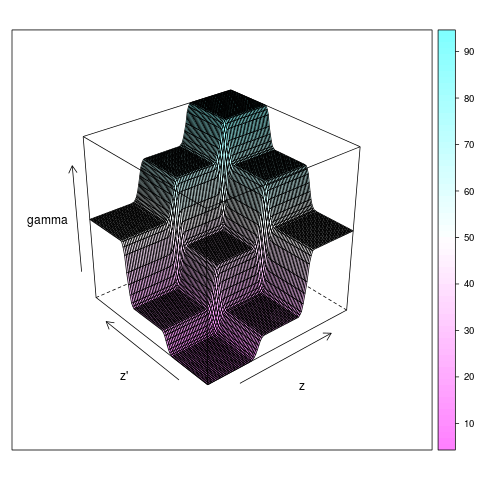
\includegraphics[width=.45\textwidth]{../FIGURES/FigGraphon-SBM-average} 
    \end{tabular}
  \end{tabular}
  
  \pause 
  \paragraph{Bayesian model averaging \refer{LaR15}:} 
  $$
  \Espt[w(u, v)] = \sum_K \Pt(K) \Espt^{SBM}_K[w(u, v)]
  $$

}

%====================================================================
\frame{ \frametitle{How to interpret a graphon?}

  \paragraph{French political blogs:}  $n = 196$ nodes \refer{LaR15}
  $$
  \includegraphics[height=.55\textheight]{../FIGURES/blogd0} 
  $$
  \ra Depicts the heterogeneity of the network.

}

%====================================================================
\section{From graphon to residual graphon}
\frame{\frametitle{Outline} \tableofcontents[currentsection]}
%====================================================================
\frame{\frametitle{Accounting for covariates  \refer{LRO15}}

  \paragraph{Data:} $Y =$ observed (binary) network, $x = $ (edge) covariates

  \pause \bigskip  \bigskip 
  \paragraph{Questions:}
  \begin{itemize}
   \item Does $x$ explain the topology of $Y$?
   \item Residual (wrt $x$) heterogeneity in $Y$?
  \end{itemize}

  \bigskip \bigskip \pause
  \paragraph{Logistic regression ($H_0$):}
  $
  \logit~P(Y_{ij} = 1) = 
  \emphase{\beta_0} + x_{ij}^\intercal \beta
  $

  \bigskip \bigskip \pause
  \paragraph{Logistic regression + graphon residual term:} $(U_i)$ iid $\sim \Ucal[0, 1]$,
  $$
  \logit~P(Y_{ij} = 1 |U_i, U_j) = 
  \emphase{\omega(U_i, U_j)} + x_{ij}^\intercal \beta
  $$

  \pause \bigskip
  \paragraph{Goodness of fit (GOF):} Check if
  $
  \omega(u, v) = \cst \qquad (= \beta_0)
  $
  }

%====================================================================
\frame{\frametitle{Goodness-of-fit as model comparison}

  \bigskip
  \paragraph{Auxiliary model $M_K$:} % $Z_i \sim \Mcal_K(1; \pi)$, $\alpha: K \times K$,
  $$
  \logit~P(Y_{ij} = 1 | U_i, U_j, K) = \emphase{\omega_K^{SBM}(U_i, U_j)} + x_{ij}^\intercal \beta.
  $$
%   \emphase{Model $M_K =$} logistic regression + $K$-class SBM residual. 
  
  \bigskip \pause
  \paragraph{Goodness of fit:} 
  $$
  \begin{array}{rclcl}
   H_0 & = & \{\text{logistic regression is sufficient}\} & = & M_1 \\
   H_1 & = & \{\text{logistic regression is not sufficient}\} & = & \bigcup_{K > 1} M_K 
  \end{array}
  $$
  GOF is a assessed if
  $$
  P(H_0|Y) = P(M_1|Y) \text{ is large.}
  $$
  
  \pause \bigskip
  \paragraph{Actually:} use $\Pt(H_0)$ and $\Pt(M_1)$.

%   \pause \bigskip \bigskip
%   \paragraph{Model averaging} yields
%   $$
%   p(\omega | Y) = \sum_k p(K|Y) \ p(\omega_K^{SBM} | Y)
%   $$

  }

%====================================================================
\frame{\frametitle{Political blog network}

  $n = 196$ blogs ($N = 19110$ pairs), 3 covariates, density $= .075$ 

  \bigskip
  \begin{tabular}{cc}
    \begin{tabular}{p{.5\textwidth}}
	 Inferred graphon (no covariate) \\ ~\\
	 \includegraphics[height=.4\textheight]{../FIGURES/blogd0} \\ ~\\
	 ~
    \end{tabular}
    & 
    \hspace{-.05\textwidth}
    \begin{tabular}{p{.5\textwidth}}
	 Residual graphon (3 covariates) \\ ~\\
	 \includegraphics[height=.4\textheight]{../FIGURES/blogd3} \\ ~\\
	 $\Pt(H_0) \simeq 10^{-172}$
    \end{tabular}
  \end{tabular}
  }

  %====================================================================
\frame{\frametitle{Florentine business}

  $n = 16$ families ($N = 120$ pairs), 3 covariates, density $= .12$ 

  \bigskip
  \begin{tabular}{cc}
    \begin{tabular}{p{.5\textwidth}}
	 Inferred graphon (no covariate) \\ ~\\
	 \includegraphics[height=.4\textheight]{../FIGURES/businessd0} \\ ~\\
	 ~
    \end{tabular}
    & 
    \hspace{-.05\textwidth}
    \begin{tabular}{p{.5\textwidth}}
	 Residual graphon (3 covariates) \\ ~\\
	 \includegraphics[height=.4\textheight]{../FIGURES/businessd3} \\ ~\\
	 $\Pt(H_0) = .991$
    \end{tabular}
  \end{tabular}
  }

%====================================================================
\frame{\frametitle{Some more examples}

\begin{centering}
\begin{tabular}{l|cccc}
 network & size ($n$) & nb. covariates ($d$) & density &$\hat{p}(H_0|Y)$ \\ 
  \hline
Blog & 196 & 3 &0.075&  3e-172 \\
Tree & 51 & 3 & 0.54 & 2e-115\\
Karate & 34 & 8 &0.14 & 3e-2 \\
Florentine (marriage) & 16 & 3 & 0.17 & 0.995 \\
Florentine (business) & 16 & 3 & 0.125 & 0.991 \\
Faux Dixon High & 248 & 17 & 0.02 & 1 \\
CKM & 219 & 39 & 0.015 & 1 \\
AddHealth 67 & 530 & 21 & 0.007& 2e-25 \\
\end{tabular}
\end{centering}
}

%====================================================================
\frame{\frametitle{Conclusion}

  \paragraph{$W$-graph}
  \begin{itemize}
   \item A well established object in the probability literature
   \item A more recent interest in the statistical community, with several theoretical results
   \item Still not very popular among practitioners
  \end{itemize}

  \pause \bigskip \bigskip 
  \paragraph{Variational Bayes inference and GOF}
  \begin{itemize}
  \item R package on \textcolor{blue}{\url{github.com/platouche/gofNetwork}} (soon on CRAN)
  \item Strongly relies on variational Bayes approximation of the posteriors. \\
  \ra VBEM asymptotically accurate for logistic regression and SBM \\
  \ra No clue about accuracy in the combined model.
  \end{itemize}

}

%====================================================================
%====================================================================
\frame[allowframebreaks]{ \frametitle{References}
{\tiny
  \bibliography{/home/robin/Biblio/BibGene}
%   \bibliographystyle{/home/robin/LATEX/Biblio/astats}
  \bibliographystyle{plain}
  }
}


%====================================================================
%====================================================================
\end{document}
%====================================================================
%====================================================================

  \begin{tabular}{cc}
    \begin{tabular}{p{.5\textwidth}}
    \end{tabular}
    & 
    \hspace{-.02\textwidth}
    \begin{tabular}{p{.5\textwidth}}
    \end{tabular}
  \end{tabular}

